\documentclass[12pt]{article}
\usepackage{graphicx}
\usepackage{wrapfig}
\usepackage{tikz}
\usepackage{ucs} 
\usepackage[T1,T2A]{fontenc}
\usepackage[utf8x]{inputenc} % Включаем поддержку UTF8  
\usepackage[russian]{babel}  % Включаем пакет для поддержки русского языка  
\usepackage{amsfonts}
\usepackage[left=1.5cm,right=1.5cm]{geometry}
\usepackage{amsmath}
\usepackage{amssymb}
\DeclareMathOperator\arctanh{arctanh}

\usetikzlibrary{decorations.markings}
\usetikzlibrary{patterns}
\usetikzlibrary{calc}
\usetikzlibrary{arrows}
\title{Задачи к 6 лекции}  
\author{Нечитаев Дмитрий}

\begin{document} 
	\maketitle
	\subsection*{Упражнение 1}
	Для уравнения
	\[\ddot{x} + x = -\epsilon x^3 \eqno(1)\]
	Нужно найти поправку второго порядка в рамках теории возмущений по малому параметру $\epsilon$ для начальных условий $x(0)=a,\;\dot{x}(0)=0$.
	
	
	Будем искать решение в виде: $x =x_0+ \epsilon x_1 + \epsilon^2 x_2$, тогда подстановка в уравнение (1) и группирование членов с одинаковыми подяками дает нам систему:
	\[\begin{cases}
	\ddot{x_0}+x_0 = 0\\
	\ddot{x_1}+x_1 = -x_0^3 \\
	\ddot{x_2} +x_2  = -3x_0^2x_1
	\end{cases}\]
	Общее решение уравнения $\ddot{x}(t)+x(t) = -y(t)$ записывается в виде:
	\[x(t) = \Big[x(0)+\int_0^{t}y(\tau)\sin\tau d\tau\Big]\cos t - \sin t \Big[\dot{x}(0)+\int_{0}^{t}y(\tau)\cos\tau d\tau\Big] \eqno(2) \] 
	Положим что $x_0(0) = a,\; x_1(0) = x_2(0) = 0,\; \dot{x_0}(0) = \dot{x_1}(0) = \dot{x_2}(0) = 0$, тогда выражения для поправок примут вид\footnote{Второе уравниение в системе было получено на лекции}:
	\[\begin{cases}
	x_0(t) = a\cos(t) \\
	x_1(t) = -\frac{a^3}{16}\Big(6t\sin t +\frac{1}{2}\cos t - \frac{1}{2}\cos 3t\Big)
	\end{cases} \eqno(3)\]
	Вычисляем $x_0^2 x_1$:
	\[x_0^2x_1 = -a^2\cos^2 t \frac{a^3}{16}\Big(6t \sin t + \frac{1}{2}\cos t - \frac{1}{2} \cos 3t\Big) = -\frac{a^5}{32}(1+\cos2t)\Big(6t \sin t + \frac{1}{2}\cos t - \frac{1}{2} \cos 3t\Big) = \]
	\[ = -\frac{a^5}{32}\Big(6t\sin t + \frac{1}{2}\cos t - \frac{1}{2}\cos3t+6t\sin t\cos 2t+\frac{1}{2}\cos t \cos 2t -\frac{1}{2}\cos3t \cos 2t\Big) = \]
	\[ = -\frac{a^5}{32}\Big(3t\sin t + 3t \sin 3t + \frac{1}{2}\cos t - \frac{1}{4}\cos 3t - \frac{1}{4}\cos 5t\Big) \eqno(4)\]
	Тогда $-3x_0^2x_1$:
	\[-3x_0^2x_1 = \frac{3a^5}{32}\Big(3t\sin t + 3t \sin 3t + \frac{1}{2}\cos t - \frac{1}{4}\cos 3t - \frac{1}{4}\cos 5t\Big) \eqno(5)\]
	Вычислим пару интегралов:
	\[I_1 = \int_0^\tau (-3x_0^2x_1) \sin t dt = \frac{3a^5}{32}\int_0^\tau dt \Big(3t\sin t + 3t \sin 3t + \frac{1}{2}\cos t - \frac{1}{4}\cos 3t - \frac{1}{4}\cos 5t\Big)\sin t = \]
	\[\frac{3a^5}{32}\int_0^\tau dt \Bigg(3t\Big(\frac{1-\cos 2t}{2} + \frac{\cos 2t - \cos 4t}{2}\Big) + \frac{\sin 2t}{4} + \frac{\sin 2t -\sin 4t}{8} + \frac{\sin 4t -\sin 6t}{8}\Bigg) = \]
	\[ \frac{3a^5}{32}\int_0^\tau dt \Bigg(3t\cdot\frac{1 - \cos 4t}{2} + \frac{\sin 2t}{4} + \frac{\sin 2t -\sin 6t}{8}\Bigg) = \frac{3a^5}{32\cdot96}\Big(72t^2-36t\sin 4t - 18 \cos 2t - 9\cos 4t + 2 \cos 6t\Big)\Bigg | _ 0 ^ \tau = \]
	\[\frac{a^5}{1024}\big(72\tau^2-36\tau\sin 4\tau - 18 \cos 2\tau - 9\cos 4\tau + 2 \cos 6\tau + 25\big) \eqno(6)\]
	\[I_2 = \int_0^\tau (-3x_0^2x_1) \cos t dt = \frac{3a^5}{32}\int_0^\tau dt \Big(3t\sin t + 3t \sin 3t + \frac{1}{2}\cos t - \frac{1}{4}\cos 3t - \frac{1}{4}\cos 5t\Big)\cos t = \]
	\[\frac{a^5}{1024}\big(24\tau+78\sin 2\tau + 3\sin 4\tau - 2\sin 6\tau - 144\tau\cos 2\tau - 36\tau\cos 4\tau\big) \eqno(7)\]
	Выражение для второй поправки:
	\[x_2(t) = \frac{a^5\sin t}{1024}\Big(24t+78\sin 2t + 3\sin 4t - 2\sin 6t - 144t\cos 2t - 36t\cos 4t\Big) - \]
	\[- \frac{a^5\cos t}{1024}\big(72t^2-36t\sin 4t - 18 \cos 2t - 9\cos 4t + 2 \cos 6t + 25\big) =\]
	\[= \frac{a^5}{1024}\Big(-72t^2\cos t+96t\sin t-36t\sin 3t + 23 \cos t -24\cos3t+\cos5t\Big)\eqno(8)\]
	Данный ответ работает при тех временах, когда вклад от второй поправки много меньше чем от первой, т.е. время до которого приближение работает хорошо определяется соотношением:
	\[\frac{a^3}{16}\cdot 6t = \epsilon \cdot \frac{72 a^5t^2}{1024} \Rightarrow t = \frac{3}{8}\cdot\frac{1024}{72}\frac{1}{a^2\epsilon} \Rightarrow t \sim \frac{1}{a^2\epsilon}\]
	
	Теперь разберемся с различными членами в ответе:
	\begin{enumerate}
		\item $72t^2\cos t$ отвечает за квадрат первой поправки к частоте
		\item $96t\sin t$ содержит вторую поправку к частоте
		\item $23\cos t$ --- поправка к амплитуде
		\item $\cos 5t, 24\cos 3t$ поправки к амплитудам для третьей и пятой гармоник
	\end{enumerate}
	
	
	\section*{Упражнение 2}
	\subsection*{Вторая поправка к частоте}
		Для получения уравнения на вторую поправку к частоте воспользуемся разложением по гармоникам. На лекции мы получили выражение,учитывающее первые поправки к амплитудам и частотам:
		\[x(t) = A\Big(1-\epsilon\frac{A^2}{32}\Big)\cos\Big(\Big[1+\epsilon\frac{3A^2}{8}\Big]t\Big) + \epsilon\frac{A^3}{32} \cos\Big(3\Big[1+\epsilon\frac{3A^2}{8}\Big]t\Big) \eqno(1)\]
		В правой части уравнения:
		\[\ddot{x}+x= -\epsilon x^3 \eqno(2)\]
		уже содержится множитель $\epsilon$, а это значит, что для учета второй попраки нам достаточно подставлять вместо $x(t)$ первое приближение решения. 
		
		Важно отметить, что исходное выражение (1) содержит только косинусы, а это значит, что в ряде фурье функции $x^3(t)$ будут содержаться только косинусы, причем дальше 9 гармоники искать бессмысленно\footnote{это следует из того, что исходное решние имеет гармоники $\omega,3\omega$, а в $x^3$ буду содержаться гармоники, частоты которых представляют собой суммы и разности частот исходной функции, т.е. максимальная частота будет $3+3+3 = 9$}. Выражение для коэффициентов фурье задается формулой:
		\[\alpha_n = \frac{1}{\pi}\int_0^{2\pi/\omega}x^3(t) \cos(n\omega t) d(\omega t) \eqno(3)\]
		Для нахождения второй поправки к частоте нам достаточно посчитать только $\alpha_1$:
		\[\alpha_1 = \frac{3A^3}{4} - \frac{3A^5}{64}\epsilon \eqno(4)\]
		Тут мы выкинули члены порядка больше 2-х, т.к. данные коэффициенты дальше умножатся на $\epsilon$.
		
		
		Пусть решение $x(t)$ является рядом фурье:
		\[x = \sum_{n=1}^{\infty} A_n \cos(n\omega t) \eqno(4)\]
		Тогда вторая производная:
		\[\ddot{x} = -\sum_{n=1}^{\infty} (n\omega)^2 A_n \cos(n\omega t) \eqno(5)\]
		Тут коэффициенты и частота являются формальными рядами по малому параметру $\epsilon$.
		
		
		Подставми данные ряды в уравнение (2) и сгруппируем все члены при первой гармонике:
		\[(1-\omega^2)A_1\cos(\omega t) = -\epsilon\alpha_1\cos(\omega t) \eqno(6)\]
		Подставляем в данное соотношение уравнения:
		\[A_1 =  A\Big(1-\epsilon\frac{A^2}{32}\Big) +\epsilon^2 A_1^{(2)} \eqno(7)\]
		\[\omega = 1 + \epsilon \frac{3A^2}{8} + \epsilon^2 \omega^{(2)} \eqno(8)\]
		После группировки слагаемых при $\epsilon^2$ получаем соотношение на $\omega^{(2)}$:
		\[-\frac{21}{128}A^5 = 2A\omega^{(2)} \Leftrightarrow \eqno(9)\]
		\[\boxed{\omega^{(2)} = -\frac{21A^4}{256}} \eqno(10)\]
		
	\subsection*{Поправки к амплитудам}
	Как уже отмечалось выше: при подстановке первого приближения в $x^3$ будут получаться гармоники равные суммам и разностям исходных, а это значит, что и следующая поправка будет содержать больше гармоник с ненулевыми амплитудами. Для вычисления поправок обратимся к формуле (3) из прошлого пункта. 
	\[\alpha_3 = \frac{A^3}{4} + \frac{3A^5}{128}\epsilon \eqno(11)\]
	\[\alpha_5 = \frac{3A^5}{128}\epsilon \eqno(12)\]
	Остальные коэффициенты либо равны нулю (четные) либо содержат величины из $O(\epsilon)$.
	
	Запишем аналоги формулы (6) для гармоник $n = 3,5$
	\[\begin{cases}
	(1-9\omega^2)A_3\cos(3\omega t) = -\epsilon \alpha_3 \cos(3\omega t) \\
	(1-25\omega^2)A_5\cos(5\omega t) = -\epsilon \alpha_3 \cos(5\omega t)
	\end{cases}, \text{где амплитуды } 
	\begin{cases}
	A_3 = \epsilon\frac{A^3}{32} + \epsilon^2 A_3^{(2)} \\
	A_5 = \epsilon^2 A_5^{(2)}
	\end{cases} \eqno(13)\]
	Собираем все слагаемые при $\epsilon^2$:
	\[\begin{cases}
	-\frac{3A^5}{16} = 8 A_3^{(2)} \\
	 \frac{3A^5}{128} = 24 A_5^{(2)}
	\end{cases} \Leftrightarrow 
	\begin{cases}
	A_3^{(2)} = -\frac{3}{128}A^5\\
	A_5^{(2)} = \frac{1}{1024}A^5
	\end{cases} \eqno(14)\]
	
	Для получения амплитуды $A_1^{(2)}$ нужно воспользоваться начальными условиями, т.е. мы должны получить, что сумма всех амплитуд $A_1,A_3,A_5$ дает нам $A$. Такое может быть только в том случае, если:
	\[A_1^{(2)} = -(A_3^{(2)}+A_5^{(2)}) =\frac{23}{1024}A^5 \eqno(15)\]
	Таким образом мы получили окончательный ответ для второго приближения:
	\[x(t) = \Big(A-\epsilon\frac{A^3}{32} + \epsilon^2 \frac{23A^5}{1024}\Big)\cos(\omega t) + \Big(\epsilon \frac{A^3}{32} - \epsilon^2 \frac{3A^5}{128}\Big)\cos(3\omega t) + \epsilon^2 \frac{A^5}{1024}\cos(5\omega t) \eqno(16)\]
	\[\omega = 1+\epsilon \frac{3A}{8} - \epsilon^2 \frac{21A^4}{256} \eqno(17)\]
	\subsection*{Разложение в ряд}
	Разложим\footnote{Попросим вольфрам посчитать это} уравнение (16) в ряд по малому параметру $\epsilon$ до $O(\epsilon^2)$:
	\[x(t) = A\cos(t) + \frac{A^3\epsilon}{32}\Big(-\cos(t)+\cos(3t)-12t\sin(t)\Big) + \] \[+\frac{A^5\epsilon^2}{1024}(23\cos(t)-72t^2\cos(t)-24\cos(3t)+\cos(5t)+96t\sin(t)-36t\sin(3t)) \eqno(18)\]
	Сравним это с выражениями (3),(8) из первого упражнения:
	\[\begin{cases}
	x_0(t) = a\cos(t) \\
	x_1(t) = -\frac{a^3}{16}\Big(6t\sin t +\frac{1}{2}\cos t - \frac{1}{2}\cos 3t\Big)
	\end{cases} \eqno(3_1)\]
	\[x_2(t) = \frac{a^5}{1024}\Big(-72t^2\cos t+96t\sin t-36t\sin 3t + 23 \cos t - 24\cos3t+\cos5t\Big)\eqno(8_1)\]
	Получаем, что разложение по гармоникам при малых временах совпадает с ответом, который был получен наивной теорией возмущений.
	\subsection*{Интегральное представление частоты}
	Существует однако и другой способ найти частоту колебаний, для этого нам потребудется вычислить значение периода, который можно получить непосредственно из уравнения движения.
	
	Перепишем соотношение (2) еще раз:
	\[\ddot{x}=-\epsilon x^3 - x \eqno(2)\] 
	Домножим данное соотношение на $\dot{x}$ и проинтегрируем:
	\[\frac{\dot{x}^2}{2} = \frac{E}{2} - \frac{x^2}{2} - \epsilon \frac{x^4}{4} \Leftrightarrow \dot{x}^2 = E - x^2 - \frac{\epsilon x^4}{2} \eqno(19)\]
	Тут константа\footnote{По сути это энергия системы, причем её значение можно определить из начальных условий} $E = A^2 - \epsilon A^4 / 2$, где $A$ --- амплитуда колебаний.
	
	
	Выражаем из ЗСЭ $\dot{x}$, разделяем переменные и интегрируем выражение для получения периода колебаний.
	\[\frac{T}{2} = \int_{-A}^{A} \frac{dx}{\sqrt{E-x^2-\epsilon x^4 /2 }} = 2\int_{0}^{A} \frac{dx}{\sqrt{E-x^2-\epsilon x^4 / 2}} \Leftrightarrow \]
	\[T = 4 \int_{0}^{A} \frac{dx}{\sqrt{E-x^2-\epsilon x^4 / 2}} \eqno(20)\]
	Возьмем инетеграл в соотношении (20), для этого подставим в него значение $E$:
	\[\int_{0}^{A}\frac{dx}{\sqrt{E-x^2-\epsilon x^4 / 2}} = \int_{0}^{A} \frac{dx}{\sqrt{(A^2-x^2)+\epsilon(A^4-x^4)/2}} = \int_{0}^{A} \frac{dx}{\sqrt{A^2-x^2}} \frac{1}{\sqrt{1+\epsilon(A^2+x^2)/2}} \approx\]
	\[\approx \int_{0}^{A} \frac{dx}{\sqrt{A^2-x^2}}\Big(1 - \frac{\epsilon}{4} (A^2+x^2) +\frac{3\epsilon^2}{32}(A^2+x^2)^2\Big) \eqno(21)\]
	Вычисляем интегралы:
	\[\int_{0}^{A}\frac{dx}{\sqrt{A^2-x^2}} = \arcsin\Big(\frac{x}{A}\Big)\Big|_{0}^{A} = \arcsin(1) = \frac{\pi}{2}\]
	\[\int_{0}^{A}\frac{(A^2+x^2)dx}{\sqrt{A^2-x^2}} = \left\{x = A\sin t \right\} = \int_{0}^{\pi/2} \frac{A^2+A^2\sin t}{A\cos t}A\cos t dt = A^2\int_{0}^{\pi/2}(1+\sin^2(t))dt = \frac{3\pi A^2}{4} \]
	\[\int_{0}^{A}\frac{(A^2+x^2)^2dx}{\sqrt{A^2-x^2}} = \left\{x = A\sin t \right\} =  A^4\int_{0}^{\pi/2}(1+\sin^2 t)^2dt = \frac{19\pi A^4}{16}\]
	Подставляем все в соотношение (21):
	\[\frac{T}{4} \approx \frac{\pi}{2} - \frac{\epsilon}{4} \cdot \frac{3\pi A^2}{4} + \frac{3\epsilon^2}{32}\cdot\frac{19\pi A^4}{16} \eqno(22)\]
	\[\frac{2\pi}{\omega} = 2\pi - \epsilon\frac{3\pi A^2}{4} + \frac{3\epsilon^2}{8}\cdot\frac{19\pi A^4}{16} \Leftrightarrow\]
	\[\frac{1}{\omega} = 1 - \epsilon\frac{3 A^2}{8} + \frac{3\epsilon^2}{16}\cdot\frac{19 A^4}{16} \eqno(23)\]
	Теперь разложим функцию $\omega$ по малому параметру:
	\[\omega = \Big(1 - \epsilon\frac{3 A^2}{8} + \frac{3\epsilon^2}{16}\cdot\frac{19 A^4}{16}\Big)^{-1} \approx 1 + \epsilon\frac{3 A^2}{8} - \frac{3\epsilon^2}{16}\cdot\frac{19 A^4}{16} + \frac{9\epsilon^2A^4}{64} = 1 +\frac{3\epsilon A^2}{8} - \frac{21\epsilon^2A^4}{256} \eqno(24)\]
	Окончательно получаем:
	\[\boxed{\omega = 1 +\frac{3\epsilon A^2}{8} - \frac{21\epsilon^2A^4}{256}} \eqno(25)\]
	\section*{Упражнение 3}
	Необходимо найти сдвиг частоты и амплитуды неосновынх гармоник из-за малого кубического ангармонизма вида:
	\[\delta U = \frac{\epsilon x^3}{3},\;\epsilon\ll1 \eqno(1)\]
	Составим уравнение движения:
	\[\ddot{x}+x = -\epsilon x^2 \eqno(2)\]
	Нулевое приближение имеет вид: $x_0(t) = A\cos(\omega t)$, тогда для рассчета первого приближения подставим в правую часть $x_0$:
	\[\ddot{x}+x = - \epsilon A^2\cos^2(\omega t) \eqno(3)\]
	Разложим функцию $x(t)$ в ряд фурье, причем данный ряд будет содержать только косинусы\footnote{Такой конфигурации мы добиваемся начальными условиями: $x(0)=A,\dot{x}(0) = 0$.}:
	\[x(t) = A_0 + \sum_{n = 1}^{\infty} A_n \cos(n\omega t) \eqno(4)\]
	Для производной:
	\[\ddot{x} = -\sum_{n = 1}^{\infty} n^2 \omega^2 A_n \cos(n\omega t)\eqno(5)\]
	Преобразуем уравнение (3):
	\[A_0 + \sum_{n = 1}^{\infty} (1-n^2\omega^2)A_n\cos(n\omega t) = -\epsilon \frac{A^2}{2}\Big(1+\cos(2\omega t)\Big) \eqno(6)\]
	Соотношение (6) дает систему из 3х уравнений, которые определяют поправки на частоту и амплитуды нулевой и второй гармоник.
	\[
	\begin{cases}
	(1-1^2\omega^2)A\cos(\omega t) = 0 \\
	A_0^{(1)} = - \frac{A^2}{2} \\
	(1-2^2\omega^2)A_2^{(1)} = - \frac{A^2}{2}
	\end{cases}
	\Leftrightarrow \begin{cases}
	\omega^{(1)} = 0 \\
	A_0^{(1)} = - \frac{A^2}{2} \\
	A_2^{(1)} =  \frac{A^2}{6}
	\end{cases} \eqno(7)
	\]
	Для определения поправки к амплитуде основной гармонике обратимся к начальным условиям: $x(0) = A,\dot{x}(0) =0$, т.е.  первый порядок дает нам решение:
	\[x(t) = -\epsilon \frac{A^2}{2} + \Big(A+\epsilon\frac{A^2}{3}\Big)\cos \omega t + \epsilon \frac{A^2}{6}\cos 2\omega t \eqno(8)\]
	Для нахождения второй поправки проводим аналогичную процедуру: подставляем в соотношение (2) выражение для первой поправки, оставляя члены, степень которых не больше 1:
	\[x^2(t) = A^2\cos^2\omega t + \frac{A^3}{3}\cos \omega t\Big(-3+3\cos \omega t + \cos 2\omega t\Big)\epsilon + O(\epsilon) \eqno(9)\]
	\[x^2(t) = \frac{A^2}{2}(1+\cos(2\omega t)) + \frac{\epsilon A^3}{2} - \frac{\epsilon 5A^3}{6}\cos\omega t + \frac{\epsilon A^3}{3}\cos 2\omega t + \frac{\epsilon A^3}{6}\cos 3 \omega t \]
	После подстановки в уравнение (2) и учета формул (4),(5) cобираем все члены при одинковых гармониках содержащие $\epsilon^2$:
	\[
	\begin{cases}
	(1-3^2\omega^2)A_3\cos(3\omega t) = -\epsilon^2 \frac{A^3}{6}\cos(3\omega t) \\
	(1-2^2\omega^2)A_2\cos(2\omega t) = -\epsilon^2 \frac{A^3}{3}\cos(2\omega t) \\
	(1-1^2\omega^2)A_1\cos(\omega t) = \epsilon^2 \frac{5A^3}{6}\cos(\omega t) \\
	(1-0^2\omega^2)A_0 = \epsilon^2 \frac{A^3}{2}
	\end{cases}
	\eqno(10)
	\]
	С последним уравнением системы все понятно:
	\[\boxed{A_0^{(2)} = \frac{A^3}{2}} \eqno(11)\]
	Посмотрим теперь на уравнение для первой гармоники:
	\[\omega = 1 + \epsilon \omega^{(1)} +\epsilon^2 \omega^{(2)}\]
	\[A_1 = A + \epsilon A_1^{(1)} +\epsilon^2 A_1^{(2)}\]
	Подставляем разложение во второе уравнение системы (10), откидывая слагаемые порядок малоскти которых больше $\epsilon^2$:
	\[(1-\omega^2)A_1 = (1-\omega)(1+\omega)(A + \epsilon A_1^{(1)} +\epsilon^2 A_1^{(2)}) = -(\epsilon \omega^{(1)} +\epsilon^2 \omega^{(2)})(2 + \epsilon \omega^{(1)} +\epsilon^2 \omega^{(2)})(A + \epsilon A_1^{(1)} +\epsilon^2 A_1^{(2)}) = \]
	\[ = -(2\epsilon\omega^{(1)}+2\epsilon^2\omega^{(2)} + \epsilon^2 (\omega^{(1)})^2)(A + \epsilon A_1^{(1)} +\epsilon^2 A_1^{(2)}) = -(2\epsilon A\omega^{(1)}+2\epsilon^2 A \omega^{(2)} + \epsilon^2 A (\omega^{(1)})^2 + 2\epsilon^2 A_1^{(1)} \omega^{(1)} )\]
	Тогда группировка слагаемых при $\epsilon^2$ и второе уравнение системы (10) дает соотношение:
	\[-\Big( 2A\omega^{(2)} + A(\omega^{(1)})^2 + 2 A_1^{(1)}\omega^{(1)} \Big) =\frac{5A^3}{6} \eqno(12)\]
	Подставляем в (12) $\omega^{(1)} = 0$ из системы (7), тогда вторая поправка к частоте примет вид:
	\[\boxed{\omega^{(2)} = -\frac{5A^2}{12}} \eqno(13)\]
	Разбираемся теперь с амлитудами 2 гармоники:
	\[(1-2^2\omega^2) = (1-2\omega)(1+2\omega) = -(1+2\epsilon^2\omega^{(2)})(3+2\epsilon^2\omega^{(2)}) = -(3+8\epsilon^2\omega^{(2)}) \eqno(14)\]
	\[(1-2^2\omega^{(2)})A_2 = -(3+8\epsilon^2\omega^{(2)})(\epsilon A_2^{(2)}+\epsilon^2 A_2^{(2)}) = -3\epsilon A_2^{(2)} - 3\epsilon^2 A_2^{(2)} \eqno(15)\]
	Тогда из системы (10) следует:
	\[\boxed{A_2^{(2)} = \frac{A^3}{9}} \eqno(16)\]
	Для третьей гармоники:
	\[(1-3^2\omega^2)\epsilon^2A_3^{(2)} = -\epsilon^2 \frac{A^3}{6} \eqno(17)\]
	\[8 A_3^{(2)} = \frac{A^3}{6} \eqno(18)\]
	\[\boxed{A_3^{(2)} = \frac{A^3}{48}} \eqno(19) \]
	Из граничных условий находим поправку к первой грамонике\footnote{Сумма всех вторых поправок к амплитудам должна быть нулевой.}:
	\[\boxed{A_1^{(2)} = -\frac{91 A^3}{144}} \eqno(20)\]
	Окончательный ответ:
	\[x(t) = \Big(-\epsilon \frac{A^2}{2} + \epsilon^2 \frac{A^3}{2}\Big) + \Big(A+\epsilon\frac{A^2}{3} - \epsilon^2\frac{91A^3}{144}\Big)\cos \omega t + \Big(\epsilon \frac{A^2}{6} + \epsilon^2 \frac{A^3}{9}\Big)\cos 2\omega t + \epsilon^2 \frac{A^3}{48} \cos 3
	\omega t\]
	\[\omega = 1 - \epsilon^2 \frac{5A^2}{12}\]
	\section*{Задача 1}
	Частица массой $m$ движется в потенциале:
	\[U(x) = U_0(\cos x - Ax) \eqno(1)\]
	На частицу также действует малая сила трения с коэффициентом $\gamma$.
	Требуется определить при каком значении $A$ возможна ненулевая средняя скорость движения частицы, найти поведение средней скорости вблизи границы диапазона.
	
	\subsection*{Поиск критического значения}
	Запишем уравнение движения частицы:
	\[\ddot{x} + \gamma\dot{x} = U_0 A + U_0 \sin x \eqno(2)\]
	Можно заменить, что подобным уравнением описывается маятник с трением, который может вращаться в вертикальной плоскости.
	\begin{figure}[h!]
		\center{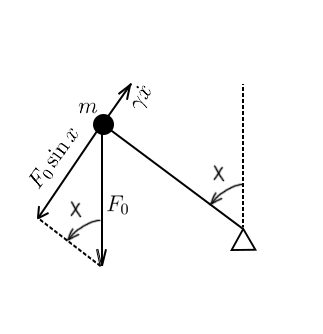
\includegraphics[scale=0.6]{pendulum.png}}
	\end{figure}
	
	Рассмотрим предельный случай движения такого маятника (нет внешней постоянной силы и нет трения), когда маятник совершает полный оборот, стартуя из вертикального положения с нулевой начальной скоростью. Понятно, что т.к. трения нет, то в конечном итоге маятник придет в конечную точку с нулевой скоростью. Запишем уравнение движения такого маятника:
	\[\ddot{x} = U_0 \sin x \eqno(3)\]
	Домножим его на $\dot{x}$ и проинтегрируем, учитывая, что $E_0 = U_0$, получим:
	\[\frac{\dot{x}^2}{2} + U_0 \cos(x) = U_0 \eqno(4)\]
	Выберем отсчет времени таким образом, чтобы в $t=0$ маятник находится в положении $x = \pi$. Пусть $x_1:= x -\pi$. Тогда $x_1(0) = 0$ и ЗСЭ принимает вид:
	\[\frac{\dot{x_1}^2}{2}-U_0\cos(x_1) = U_0 \eqno(5)\]
	Выражаем $\dot{x_1}$, заделяем переменные и интегрируем:
	\[t = \frac{1}{\sqrt{2}}\int_{0}^{x_1(t)} \frac{dx}{\sqrt{U_0 + U_0 \cos(x)}} = \frac{1}{\sqrt{4U_0}} \int_{0}^{x_1(t)}\frac{dx}{\cos(x/2)} = \left\{ \sin(x/2) = \tanh(z) \right\} = \]
	\[ = \frac{1}{\sqrt{U_0}} \int_0^{\arctanh \sin \frac{x_1}{2}} dz = \frac{1}{\sqrt{U_0}} \arctanh \sin \frac{x_1}{2} \eqno(6)\]
	\[\boxed{x = \pi + 2 \arcsin \tanh \sqrt{U_0}t  }\eqno(7)\]
	\[\dot{x} = 2\sqrt{U_0} \frac{1}{\cosh^2(t\sqrt{U_0}) \sqrt{1-\tanh^2(t\sqrt{U_0}})} = \frac{2\sqrt{U_0}}{\cosh(t\sqrt{U_0})} \eqno(8)\]
	
	
	Пусть теперь есть трение и внешняя сила. Записутим маятник из верхнего положения без начальной скорости, после совершения оборота скорость должна быть ненулевой. Рассмотрим приращение энергии в таком движении, считая, что сила трения и внешняя сила малы.
	\[\frac{v_\text{конечная}^2}{2} - 0 = \int_0^{2\pi}U_0A dx - \int_0^{2\pi} \gamma \dot{x} dx = \int_{-\infty}^{\infty}U_0A \dot{x} dt - \int_{-\infty}^{\infty} \gamma \dot{x}^2 dt = \]
	\[= U_0A \int_{-\infty}^{\infty} \frac{2\sqrt{U_0}}{\cosh(t\sqrt{U_0})} dt - 4\gamma U_0 \int_{-\infty}^{\infty} \frac{dt}{\cosh^2(t\sqrt{U_0})} = 2U_0A\pi - 8\gamma \sqrt{U_0} \ge 0  \eqno(9) \]
	Критическое значение параметра $A$:
	\[\boxed{A = \frac{4\gamma}{\pi\sqrt{U_0}}}
	\eqno(10)\]
	
	Исходя из формулы (10) можно заключить, что наше предположение о малости $A$ было правильным, причем стоит заметить, что если поменять знак в выражении для $A$, то все рассуждения будут аналогичными, просто маятник будет двигаться в противоположную сторону.
	
	\subsection*{Исследование вблизи критического положения}
	Пусть теперь частица движется в потенциале:
	\[U(x) = U_0\Big(\cos x - \frac{4\gamma}{\pi \sqrt{U_0}}x\Big)\ \eqno(1)\]
	В прошлом пункте задачи мы показали, что при в таком потенциале воможно инфинитное движение при наличии трения.
	
	Рассмотрим движение системы вблизи положения $x=0$, пренебрегая работой силы терения запишем ЗСЭ:
	\[U_0 = \frac{\dot{x}^2}{2} + U_0\cos x - \frac{4\gamma \sqrt{U_0}}{\pi}x \approx \frac{\dot{x}^2}{2} + U_0\Big(1-\frac{x^2}{2}\Big) - \frac{4\gamma \sqrt{U_0}}{\pi}x \eqno(2) \]
	Приближенное выражение будет иметь вид:
	\[\dot{x} = \sqrt{U_0}\sqrt{x^2+\frac{8\gamma \sqrt{U_0}}{\pi}x} \eqno(3)\]
	Введем параметр $\alpha = \frac{4\gamma\sqrt{U_0}}{\pi}$, тогда уравнение (3) перепишется в виде:
	\[\frac{dx}{\sqrt{x^2+2\alpha}} = \sqrt{U_0} dt\]
	\[\frac{dx}{\sqrt{(x+\alpha)^2-\alpha^2}} = \sqrt{U_0}dt\]
	Если пренебречь слагаемым $\alpha^2$, то при интегрировании от 0 до величины\footnote{Выбор конечного значнения в интеграле выбирается так, чтобы приближение $cos(x)\approx (1-x^2/2)$, а с ним и сохранение энергии перестали работать} порядка $1$,то получим, что существенную часть времени частица находится в окрестности максимума потенциала:
	\[t_1 \approx \frac{1}{\sqrt{U_0}}\int_0^1 \frac{dx}{(x+\alpha)} \approx \frac{1}{\sqrt{U_0}}\ln\Big(\frac{1+\alpha}{\alpha}\Big)\]
	По аналогии находим $t_2$ --- время нахождения частицы в окрестности максимума $x = 2\pi$.
	\[t_2 = t_1 \Rightarrow T = t_1 + t_2 + t_3 \eqno(4)\]
	Тут $t_3$ --- время прохождения частицы от положения $\epsilon$ до $2\pi - \epsilon$, $\epsilon \sim 1$ 
	
	
	Тогда среднюю скорость движения частицы можно оценить соотношением:
	\[<V> = \frac{2\pi}{2t_1} = \frac{\pi\sqrt{U}}{\ln\big(\frac{1+\alpha}{\alpha}\big)} \approx -\frac{\pi\sqrt{U}}{\ln(\alpha)} = -\pi\sqrt{U}\ln\Big(\frac{4\gamma\sqrt{U_0}}{\pi}\Big)^{-1}\]
\end{document}